\documentclass[aspectratio=169, 11pt]{beamer}

\usetheme{metropolis}
\usepackage{amsmath, amssymb}
\usepackage{booktabs}
\usepackage{tikz}
\usetikzlibrary{arrows.meta, positioning, calc, shapes.geometric}
\usepackage{xcolor}
\usepackage{hyperref}

\definecolor{vera}{HTML}{E8607A}
\definecolor{marcus}{HTML}{5B9BD5}
\definecolor{theo}{HTML}{E8A838}
\definecolor{elliot}{HTML}{7B68C8}
\definecolor{rafael}{HTML}{4BAE8A}
\definecolor{dex}{HTML}{E07B54}
\definecolor{darkbg}{HTML}{23373B}

\title{Simulating Mate Selection with LLM-Powered Agent-Based Models}
\subtitle{A Computational Social Science Approach}
\author{Se\c{c}kin \"Ozbek}
\date{April 2026}
\institute{}

\begin{document}

% ============================================================
% TITLE
% ============================================================
\maketitle

% ============================================================
% OUTLINE
% ============================================================
\begin{frame}{Outline}
\tableofcontents
\end{frame}

% ============================================================
\section{Research Question}
% ============================================================

\begin{frame}{Research Question}
\begin{center}
\Large\textbf{Can LLM agents simulate empirically grounded\\mate selection dynamics?}
\end{center}

\vspace{1em}

Three sub-questions:
\begin{enumerate}
    \item Can parameterized personality profiles produce \textbf{psychologically plausible} dialogue?
    \item Do rule-based scoring functions \textbf{faithfully operationalize} published theories?
    \item Does adding \textbf{agentic tool use} produce emergent dynamics beyond scripted simulation?
\end{enumerate}
\end{frame}

\begin{frame}{What This Is (and Isn't)}
\begin{columns}[T]
\begin{column}{0.48\textwidth}
\textbf{Agent-Based Model (ABM)}\\[0.5em]
Computational social science tradition (Gilbert \& Troitzsch, 2005). Agents have explicit psychological parameters. Emergent dynamics result from parameter interactions, not LLM priors.
\end{column}
\begin{column}{0.48\textwidth}
\textbf{Not ``Agentic AI''}\\[0.5em]
The LLM is a \textit{dialogue engine} --- it translates Big Five scores and attachment rules into natural language. All scoring is rule-based Python, not LLM-driven.
\end{column}
\end{columns}

\vspace{1.5em}
\begin{center}
\textit{The agentic upgrade adds tool-use so ABM actors become AI agents\\with bounded autonomy --- but cannot modify the scoring functions.}
\end{center}
\end{frame}

% ============================================================
\section{Theoretical Framework}
% ============================================================

\begin{frame}{Eight Theories, One Simulation}
\small
\begin{tabular}{@{}p{3.2cm}p{4.5cm}p{4.8cm}@{}}
\toprule
\textbf{Theory} & \textbf{Source} & \textbf{Operationalization} \\
\midrule
Five-Factor Model & Costa \& McCrae (1992) & Agent personality vectors \\
Attachment Theory & Bowlby (1969); Hazan \& Shaver (1987) & 4-style taxonomy + compatibility matrix \\
SVR Theory & Murstein (1970) & 3-stage selection: $S{=}0.3, V{=}0.4, R{=}0.3$ \\
Necessities vs.\ Luxuries & Li et al.\ (2002) & Trait budget model \\
Assortative Mating & Thiessen \& Gregg (1980) & Cosine similarity on trait vectors \\
Four Horsemen & Gottman et al.\ (1998) & Personality-derived risk proxies \\
5:1 Ratio & Gottman (1994) & Stability prediction threshold \\
Sexual Strategies & Buss \& Schmitt (1993) & Strategy alignment penalty \\
\bottomrule
\end{tabular}
\end{frame}

% ============================================================
\section{Mathematical Foundations}
% ============================================================

\begin{frame}{Compatibility Scoring}
\textbf{Cosine similarity} for Big Five and trait vectors:
\[
\text{sim}(\mathbf{a}, \mathbf{b}) = \frac{\mathbf{a} \cdot \mathbf{b}}{\|\mathbf{a}\| \, \|\mathbf{b}\|}
\]

\textbf{Overall compatibility} (weighted sum):
\[
C = \underbrace{0.25}_{\text{Big Five}} \cdot \text{sim}_{\text{B5}} + \underbrace{0.20}_{\text{Traits}} \cdot \text{sim}_{\text{T}} + \underbrace{0.35}_{\text{Attach.}} \cdot A_{ij} + \underbrace{0.20}_{\text{Strategy}} \cdot S
\]

\vspace{0.5em}
\small
Weight justification:
\begin{itemize}
    \item Attachment compatibility ($0.35$): strongest predictor per Hazan \& Shaver (1987)
    \item Big Five similarity ($0.25$): moderate predictor in assortative mating literature
    \item Strategy alignment ($0.20$): mismatch is costly per Buss \& Schmitt (1993)
    \item Trait similarity ($0.20$): secondary to attachment per Li et al.\ (2002)
\end{itemize}
\end{frame}

\begin{frame}{Attachment Compatibility Matrix}
\small
Empirical attachment compatibility $A_{ij} \in [0, 1]$:

\vspace{0.5em}
\begin{tabular}{@{}lccccc@{}}
\toprule
 & \textbf{Secure} & \textbf{Anxious} & \textbf{Dismiss.} & \textbf{Fearful} \\
\midrule
\textbf{Secure}    & 0.95 & 0.65 & 0.60 & 0.50 \\
\textbf{Anxious}   &      & 0.40 & \alert{0.25} & 0.30 \\
\textbf{Dismissive} &     &      & 0.35 & 0.30 \\
\textbf{Fearful}   &      &      &      & 0.20 \\
\bottomrule
\end{tabular}

\vspace{1em}
\alert{0.25}: The anxious--avoidant trap (Kirkpatrick \& Davis, 1994).\\
Anxious partner pursues $\rightarrow$ avoidant withdraws $\rightarrow$ pursuit intensifies $\rightarrow$ collapse.
\end{frame}

\begin{frame}{SVR Theory: Three-Stage Selection}
Murstein's (1970) Stimulus--Value--Role model:

\begin{align*}
\text{Stimulus} &= \frac{1}{2}\left(\bar{O}_{\text{obs}}(A \to B) + \bar{O}_{\text{obs}}(B \to A)\right) & \text{weight } 0.30 \\[0.5em]
\text{Value} &= \text{sim}_{\text{B5}}(A, B) & \text{weight } 0.40 \\[0.5em]
\text{Role} &= 0.7 \cdot \mathbb{1}[\text{strategy match}] + 0.3 \cdot (1 - \tfrac{|C_A - C_B|}{200}) & \text{weight } 0.30
\end{align*}

\vspace{0.5em}
where $\bar{O}_{\text{obs}}$ averages attractiveness, humor, and extraversion (the ``observable'' traits in a bar setting), and $C_A, C_B$ are conscientiousness scores.

\[
\text{SVR}_{\text{total}} = 0.30 \cdot S + 0.40 \cdot V + 0.30 \cdot R
\]
\end{frame}

\begin{frame}{Gottman's Four Horsemen: Operationalization}
Personality-derived proxies (all clamped to $[0, 1]$):

\begin{align*}
\text{Criticism} &= \min\!\Big(1,\; \bar{N} \cdot 1.3 \cdot (1 - \bar{A})\Big) \\[0.3em]
\text{Contempt} &= \min\!\Big(1,\; (1 - A_{ij}) \cdot 0.8 + \bar{N} \cdot 0.3\Big) \\[0.3em]
\text{Defensiveness} &= \min\!\Big(1,\; \bar{N} \cdot 0.7 + (1 - \bar{A}) \cdot 0.5\Big) \\[0.3em]
\text{Stonewalling} &= \min\!\Big(1,\; (1 - \bar{S}) \cdot 0.5 + 0.4 \cdot \mathbb{1}[\text{avoidant}]\Big)
\end{align*}

where $\bar{N} = \frac{N_1 + N_2}{200}$, $\bar{A} = \frac{A_1 + A_2}{200}$, $\bar{S} = \frac{S_1 + S_2}{200}$ (stability).

\vspace{0.5em}
\textbf{5:1 Ratio} (Gottman, 1994): Stable couples maintain $\geq 5$ positive interactions per negative one.
\end{frame}

\begin{frame}{Stability Prediction}
\[
\text{Stability} = \min\!\bigg(100,\; \max\!\Big(0,\; 40C + R_{\text{bonus}} + 30(1 - \bar{H})\Big)\bigg)
\]

where:
\begin{itemize}
    \item $C$ = overall compatibility score
    \item $\bar{H}$ = mean of Four Horsemen scores
    \item $R_{\text{bonus}}$: $30$ if ratio $\geq 5$, $20$ if $\geq 3$, $10$ if $\geq 1$, else $0$
\end{itemize}

\vspace{1em}
\begin{tabular}{@{}lll@{}}
\toprule
\textbf{Score} & \textbf{Prediction} & \textbf{Action} \\
\midrule
$\geq 75$ & Likely stable & --- \\
$50$--$74$ & At risk & Monitor \\
$< 50$ & Likely to dissolve & Intervene \\
\bottomrule
\end{tabular}
\end{frame}

% ============================================================
\section{System Architecture}
% ============================================================

\begin{frame}{Two Operating Modes}
\begin{columns}[T]
\begin{column}{0.45\textwidth}
\textbf{Scripted Mode}\\[0.5em]
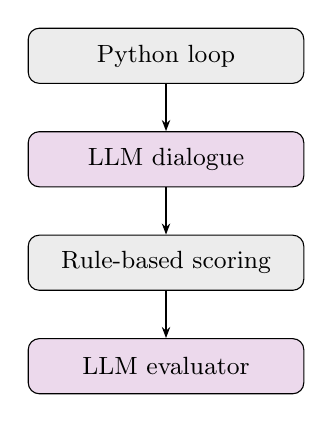
\begin{tikzpicture}[
    node distance=0.6cm,
    every node/.style={draw, rounded corners, minimum width=3.5cm, minimum height=0.7cm, font=\small, align=center},
    arr/.style={-{Stealth[length=4pt]}, thick}
]
\node (loop) [fill=gray!15] {Python loop};
\node (llm1) [below=of loop, fill=violet!15] {LLM dialogue};
\node (score) [below=of llm1, fill=gray!15] {Rule-based scoring};
\node (llm2) [below=of score, fill=violet!15] {LLM evaluator};
\draw[arr] (loop) -- (llm1);
\draw[arr] (llm1) -- (score);
\draw[arr] (score) -- (llm2);
\end{tikzpicture}
\end{column}
\begin{column}{0.45\textwidth}
\textbf{Agentic Mode}\\[0.5em]
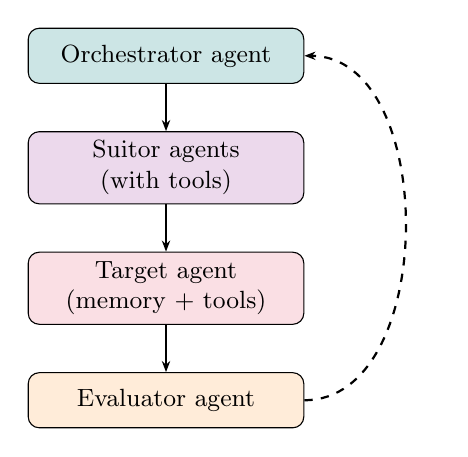
\begin{tikzpicture}[
    node distance=0.6cm,
    every node/.style={draw, rounded corners, minimum width=3.5cm, minimum height=0.7cm, font=\small, align=center},
    arr/.style={-{Stealth[length=4pt]}, thick}
]
\node (orch) [fill=teal!20] {Orchestrator agent};
\node (suit) [below=of orch, fill=violet!15] {Suitor agents\\(with tools)};
\node (vera) [below=of suit, fill=vera!20] {Target agent\\(memory + tools)};
\node (eval) [below=of vera, fill=orange!15] {Evaluator agent};
\draw[arr] (orch) -- (suit);
\draw[arr] (suit) -- (vera);
\draw[arr] (vera) -- (eval);
\draw[arr, dashed] (eval.east) to[out=0,in=0] (orch.east);
\end{tikzpicture}
\end{column}
\end{columns}
\end{frame}

\begin{frame}{Agentic Tool Use}
\small
\begin{tabular}{@{}llp{6.5cm}@{}}
\toprule
\textbf{Agent} & \textbf{Tool} & \textbf{Function} \\
\midrule
\multirow{3}{*}{Suitor} & \texttt{check\_compatibility} & Queries \texttt{compatibility.py} + \texttt{selection.py}; returns scores mid-conversation \\
 & \texttt{change\_strategy} & Switches long-term $\leftrightarrow$ short-term based on signals \\
 & \texttt{read\_body\_language} & Word-list sentiment heuristic on Vera's last response \\
\midrule
Target (Vera) & \texttt{end\_conversation\_early} & Exits encounter; sets early\_exit flag \\
\midrule
\multirow{2}{*}{Orchestrator} & \texttt{introduce\_event} & Injects environmental events (loud music, last call, etc.) \\
 & \texttt{call\_evaluator} & Invokes Gottman analysis on chosen pair \\
\bottomrule
\end{tabular}

\vspace{0.8em}
\textbf{Key constraint}: Agents can \textit{query} scoring functions but cannot \textit{modify} them.\\
The ABM parameters are the ground truth; agents adapt \textit{within} the rules.
\end{frame}

\begin{frame}{Fatigue Mechanic}
Vera's fatigue increases linearly across encounters:
\[
f_i = \frac{i}{n - 1}, \quad i \in \{0, 1, \ldots, n-1\}
\]

For $n = 5$ suitors: $f = 0.0, 0.25, 0.50, 0.75, 1.0$

\vspace{0.5em}
\begin{tabular}{@{}ll@{}}
\toprule
\textbf{Fatigue} & \textbf{Behavioral effect} \\
\midrule
$0.00$--$0.25$ & Fresh and genuinely open \\
$0.26$--$0.50$ & Patience for small talk shortening \\
$0.51$--$0.75$ & Needs something genuinely interesting \\
$0.76$--$1.00$ & Guarded; generic openers get brief responses \\
\bottomrule
\end{tabular}

\vspace{0.8em}
\textit{Implication}: Suitor 1 (Marcus) has an inherent advantage. Suitor 5 (Dex) must overcome both fatigue and Vera's accumulated comparison set.
\end{frame}

% ============================================================
\section{Agent Profiles}
% ============================================================

\begin{frame}{The Cast}
\small
\begin{tabular}{@{}l@{\hspace{4pt}}c@{\hspace{4pt}}c@{\hspace{4pt}}c@{\hspace{4pt}}c@{\hspace{4pt}}c@{\hspace{4pt}}l@{\hspace{4pt}}l@{}}
\toprule
\textbf{Agent} & \textbf{O} & \textbf{C} & \textbf{E} & \textbf{A} & \textbf{N} & \textbf{Attachment} & \textbf{Strategy} \\
\midrule
\textcolor{vera}{\textbf{Vera}} (Target) & 85 & 78 & 70 & 62 & 42 & Secure & Long-term \\
\textcolor{marcus}{Marcus} (Architect) & 72 & 82 & 65 & 75 & 28 & Secure & Long-term \\
\textcolor{theo}{Theo} (Performer) & 78 & 48 & 92 & 70 & 78 & Anxious & Short-term \\
\textcolor{elliot}{Elliot} (Analyst) & 90 & 75 & 32 & 42 & 35 & Dismissive & Long-term \\
\textcolor{rafael}{Rafael} (Romantic) & 82 & 52 & 74 & 82 & 72 & Anxious & Long-term \\
\textcolor{dex}{Dex} (Drifter) & 88 & 38 & 60 & 58 & 68 & Fearful & Short-term \\
\bottomrule
\end{tabular}

\vspace{1em}
Design: all four attachment styles represented. Two short-term strategists (Theo, Dex) create mismatch tension with Vera's long-term orientation.
\end{frame}

\begin{frame}{Predicted Pairings (Rule-Based)}
\begin{tabular}{@{}llccc@{}}
\toprule
\textbf{Pair} & \textbf{Compat.} & \textbf{Attach.} & \textbf{Stability} & \textbf{Prediction} \\
\midrule
Vera $\times$ \textcolor{marcus}{Marcus} & 98\% & 95\% & 94 & Likely stable \\
Vera $\times$ \textcolor{rafael}{Rafael} & 84\% & 65\% & 64 & At risk \\
Vera $\times$ \textcolor{theo}{Theo} & 75\% & 65\% & 59 & At risk \\
Vera $\times$ \textcolor{elliot}{Elliot} & 83\% & 60\% & 61 & At risk \\
Vera $\times$ \textcolor{dex}{Dex} & 70\% & 50\% & 51 & At risk \\
\bottomrule
\end{tabular}

\vspace{1em}
Marcus dominates: two secure-attached, long-term strategists with high conscientiousness. Assortative mating at its most predictable.

\vspace{0.5em}
\textit{Question}: Does the agentic simulation confirm or disrupt these predictions?
\end{frame}

% ============================================================
\section{Cost Engineering}
% ============================================================

\begin{frame}{Dual-Model Strategy}
\small
\begin{tabular}{@{}lllrl@{}}
\toprule
\textbf{Mode} & \textbf{Models} & \textbf{Calls/run} & \textbf{Cost/run} & \textbf{Notes} \\
\midrule
Scripted & Sonnet & 17 & \$0.09 & Baseline \\
Scripted + annotate & Sonnet & 32 & \$0.16 & +15 annotations \\
Agentic (na\"ive) & Sonnet only & $\sim$50 & \$0.60 & No optimization \\
\textbf{Agentic (optimized)} & \textbf{Sonnet + Haiku} & \textbf{$\sim$50} & \textbf{\$0.17} & \textbf{Dual-model + caching} \\
Agentic + annotate & Sonnet + Haiku & $\sim$65 & \$0.19 & +15 Haiku annotations \\
\bottomrule
\end{tabular}

\vspace{1em}
\textbf{Three optimizations}:
\begin{enumerate}
    \item Sonnet for dialogue, Haiku for tool-continuation turns ($-60\%$)
    \item Prompt caching: 90\% discount on repeated system prompts ($-25\%$)
    \item \texttt{max\_tool\_calls=2} cap prevents runaway loops
\end{enumerate}

\vspace{0.5em}
Net result: agentic mode costs $2\times$ scripted, not $7\times$.
\end{frame}

% ============================================================
\section{Limitations \& Future Work}
% ============================================================

\begin{frame}{Limitations}
\begin{enumerate}
    \item \textbf{Four Horsemen are trait-derived proxies}. Gottman used the Specific Affect Coding System (SPAFF) on live video. We derive from personality scores --- a modeling simplification.
    
    \item \textbf{No longitudinal dynamics}. Gottman's research tracked newlyweds over 6 years. We model a single evening.
    
    \item \textbf{Binary mating strategies}. Real strategies exist on a continuum; long-term/short-term is a simplification of SST.
    
    \item \textbf{Sentiment heuristic}. \texttt{read\_body\_language()} uses bag-of-words, not pragmatic analysis.
    
    \item \textbf{Memory as text}. Vera's cross-encounter memory is serialized into the system prompt; no episodic structure.
\end{enumerate}
\end{frame}

\begin{frame}{Future Work}
\begin{itemize}
    \item \textbf{Multi-round simulation}: second dates, relationship evolution over time
    \item \textbf{SPAFF-inspired scoring}: analyze conversation text for Horsemen signals instead of deriving from traits
    \item \textbf{Variable agent pools}: parameterized generation of $n$ agents from distributions
    \item \textbf{Longitudinal tracking}: stability score trajectories across simulated weeks/months
    \item \textbf{Validation}: compare simulation predictions against empirical datasets (speed dating studies, e.g.\ Fisman et al., 2006)
\end{itemize}
\end{frame}

% ============================================================
\section{References}
% ============================================================

\begin{frame}[allowframebreaks]{References}
\small
\begin{itemize}
    \item Bowlby, J. (1969). \textit{Attachment and Loss: Vol.\ 1. Attachment}. Basic Books.
    \item Buss, D.\ M., \& Schmitt, D.\ P. (1993). Sexual strategies theory: An evolutionary perspective on human mating. \textit{Psychological Review}, 100(2), 204--232.
    \item Carrere, S., \& Gottman, J.\ M. (1999). Predicting divorce among newlyweds from the first three minutes of a marital conflict discussion. \textit{Family Process}, 38(3), 293--301.
    \item Costa, P.\ T., \& McCrae, R.\ R. (1992). \textit{Revised NEO Personality Inventory (NEO-PI-R) and NEO Five-Factor Inventory (NEO-FFI) Professional Manual}. Psychological Assessment Resources.
    \item Gilbert, N., \& Troitzsch, K. (2005). \textit{Simulation for the Social Scientist} (2nd ed.). Open University Press.
    \item Gottman, J.\ M. (1994). \textit{What Predicts Divorce? The Relationship Between Marital Processes and Marital Outcomes}. Lawrence Erlbaum.
    \item Gottman, J.\ M., Coan, J., Carrere, S., \& Swanson, C. (1998). Predicting marital happiness and stability from newlywed interactions. \textit{Journal of Marriage and the Family}, 60(1), 5--22.
    \item Hazan, C., \& Shaver, P. (1987). Romantic love conceptualized as an attachment process. \textit{Journal of Personality and Social Psychology}, 52(3), 511--524.
    \item Kirkpatrick, L.\ A., \& Davis, K.\ E. (1994). Attachment style, gender, and relationship stability: A longitudinal analysis. \textit{Journal of Personality and Social Psychology}, 66(3), 502--512.
    \item Li, N.\ P., Bailey, J.\ M., Kenrick, D.\ T., \& Linsenmeier, J.\ A.\ W. (2002). The necessities and luxuries of mate preferences. \textit{Journal of Personality and Social Psychology}, 82(6), 947--955.
    \item Murstein, B.\ I. (1970). Stimulus--Value--Role: A theory of marital choice. \textit{Journal of Marriage and the Family}, 32(3), 465--481.
    \item Thiessen, D., \& Gregg, B. (1980). Human assortative mating and genetic equilibrium: An evolutionary perspective. \textit{Ethology and Sociobiology}, 1(2), 111--140.
\end{itemize}
\end{frame}

% ============================================================
\begin{frame}[standout]
    \Large Demo: \texttt{py -3.9 src/main.py --agentic --serve}
    
    \vspace{1em}
    \normalsize
    \url{https://seckinozbek1.github.io/dating-game-sim/viewer/retro.html}
\end{frame}

\end{document}
